\mychapter{3}{Preliminary results}
%
% This section should include your research efforts. Appropriate discussion and methods are important; you should show how you can perform all of the necessary techniques and methods. Please embed figures into the text and include a brief legend. Figures and Tables must be absolutely clear and visible. 
%
%%%%%%%%%%%%%%%%%%%%%%%%%%%%%%%%%%%%%%%%%%%%%%%%%%%%%%%%%%%%%%%%%%%%%%%%%%%%%%%%%%%%
%%%%%%%%%%%%%%%%%%%%%%%%%%%%%%%%%%%%%%%%%%%%%%%%%%%%%%%%%%%%%%%%%%%%%%%%%%%%%%%%%%%%
\section*{Background}
%%%%%%%%%%%%%%%%%%%%%%%%%%%%%%%%%%%%%%%%%%%%%%%%%%%%%%%%%%%%%%%%%%%%%%%%%%%%%%%%%%%%
%%%%%%%%%%%%%%%%%%%%%%%%%%%%%%%%%%%%%%%%%%%%%%%%%%%%%%%%%%%%%%%%%%%%%%%%%%%%%%%%%%%%

%%%%%%%%%%%%%%%%%%%%%%%%%%%%%%%%%%%%%%%%%%%%%%%%%%%%%%%%%%%%%%%%%%%%%%%%%%%%%%%%%%%%
\subsection*{Intracranial Encephalography (iEEG)}
%%%%%%%%%%%%%%%%%%%%%%%%%%%%%%%%%%%%%%%%%%%%%%%%%%%%%%%%%%%%%%%%%%%%%%%%%%%%%%%%%%%%
The electrical currents of the brain were first discovered by Richard Caton from the cortices of rabbits \citep{Caton1875}, but the the electroencephalograph (EEG) became a mainstay of brain research when Hans Berger discovered the alpha wave \citep{Berger1929}. Since then, many other brain rhythms have been described, such as the slow waves, spindles, and ripples described in the introduction as well as many rhythms, less associated with SWS such theta, beta, and gamma. For obvious reasons, most EEG studies of humans utilize non-invasive scalp electrodes, but if serious health circumstances arise such as focal epilepsy, it may be necessary to record from the brain intracranially \citep{Jasper1949}. Whereas, brain signals must conduct through CSF, skull, muscle, skin, etc. to reach scalp electrodes, iEEG electrodes are typically in direct contact with brain tissue. Therefore, signals are significantly stronger, contain less artifact, and have much greater spatial resolution. Nevertheless, iEEG measures the net potential difference integrated over a particular area (referenced to another), and is composed of a complex mixture of every excitable membrane and corresponding transmembrane currents in the electrodes vicinity from fast-spiking interneurons to slowly-fluctuating Ca$^{2+}$ currents in glia \citep{Buzsaki2012}.


%[Cite: Origins of extracellular feilds - Buszaki, Anastassiou, & Koch, 2012]

%%%%%%%%%%%%%%%%%%%%%%%%%%%%%%%%%%%%%%%%%%%%%%%%%%%%%%%%%%%%%%%%%%%%%%%%%%%%%%%%%%%%
\subsection*{Network Connectivity}
%%%%%%%%%%%%%%%%%%%%%%%%%%%%%%%%%%%%%%%%%%%%%%%%%%%%%%%%%%%%%%%%%%%%%%%%%%%%%%%%%%%%
Functional connectivity involves characterizing the statistical relationship between the signals in brain components (nodes), while anatomical connectivity describes the way these nodes are physically connected \citep{Rubinov2010}. On the other hand, a mechanistic account of brain activity involves describing how the functional connectivity emerges out of its anatomical substrate \citep{Honey2009}. This so called effective connectivity consists of a model describing how the anatomical elements affect each other \citep{Bullmore2009}.

Common measures of functional connectivity are zero-lag correlation, spectral coherence, and phase-amplitude coupling. Typically the measure is computed for all pairs of nodes

High values of functional connectivity generally mean that the signals are similar, which is 

entail a fully connected network, effective networks provide a sparser.

% One of the simplest ways this could be accomplished is with a system of linear equations modeling a signals as the superposition of its input signals. Although, neurons are not linear systems and form vast networks, sometimes with very remote connections.

%%%%%%%%%%%%%%%%%%%%%%%%%%%%%%%%%%%%%%%%%%%%%%%%%%%%%%%%%%%%%%%%%%%%%%%%%%%%%%%%%%%%
\subsection*{Traveling waves}
%%%%%%%%%%%%%%%%%%%%%%%%%%%%%%%%%%%%%%%%%%%%%%%%%%%%%%%%%%%%%%%%%%%%%%%%%%%%%%%%%%%%
By describing how signals propagate from one region to another, traveling waves can be regarded as effective connectivity. Superficial layers of the cortex have substantial recurrent connectivity.
%“Therefore, the dynamical organization of rs-fMRI and its relation to brain states may manifest more fundamentally in spatiotemporal trajectories than changes in correlation structure.” (Mitra, 2018). “... our results suggest that—at least for the frequencies and regions we examined—the precise frequency of an oscillation could most closely relate to broad physiological factors such as the direction of wave propagation...The coexistence of traveling waves and CFC suggests that spatial bands of high-frequency neural activity move across the human cortex during behavior (Bahramisharif et al., 2013)” (Zhang, 2018)

%%%%%%%%%%%%%%%%%%%%%%%%%%%%%%%%%%%%%%%%%%%%%%%%%%%%%%%%%%%%%%%%%%%%%%%%%%%%%%%%%%%%
%%%%%%%%%%%%%%%%%%%%%%%%%%%%%%%%%%%%%%%%%%%%%%%%%%%%%%%%%%%%%%%%%%%%%%%%%%%%%%%%%%%%
\section*{Methods}
%%%%%%%%%%%%%%%%%%%%%%%%%%%%%%%%%%%%%%%%%%%%%%%%%%%%%%%%%%%%%%%%%%%%%%%%%%%%%%%%%%%%
%%%%%%%%%%%%%%%%%%%%%%%%%%%%%%%%%%%%%%%%%%%%%%%%%%%%%%%%%%%%%%%%%%%%%%%%%%%%%%%%%%%%
\subsection*{Data preprocessing}
Data were re-referenced by to the common average of all electrodes located in brain matter. The common average was chosen so that any global artifacts would be removed and elected over local re-referencing schemes which are more likely to disrupt spatial correlations between neighboring electrodes. Since sleep records are many hours in duration, all records were low-pass filtered and down sampled (\textsf{MATLAB's} \texttt{resample} function) from 5000 Hz to 2000 Hz to reduce storage and computational burden. Bandpass filters were used for various purposes such as artifact detection and analysis of sleep rhythms; these were implemented forward and reverse finite impulse response filter (\textsf{MATLAB's} \texttt{filtfilt} and \texttt{fir1s} functions).

Artifact's due to epileptiform discharges were detected as unusual high power in low and high frequency bands \citep[see]{Gelinas2016}. Detection of waveforms, such as slow waves or spindles, was accomplished by: (1) bandpass filtering data for the particular band, (2) applying the hilbert transform to the filtered data, (3) detecting all local maxima, i.e. peaks, and (4) choosing all peaks above the 99$^{th}$ particular percentile.

Subject MRI and CT scans were co-registered a common MNI space. Then to determine the location of electrodes, round areas of high intensity in the CT scan were manually selected and clinical notes were used correctly match the channel's location to its recording label. Freesurfer was used to acquire a 3D surface mesh rendering of the cortex.  

\subsubsection*{Spatial embedding of electrodes}
The majority of work on traveling waves have described these phenomena with respect to Euclidean space. While this is reasonable for rodents, this may be an overly simplistic assumption due to the extensive gyrification of the human brain. To improve on this apparent short-coming, I elected to develop a method utilizing geodesic distance, or the shortest distance between points on a convoluted surface.

Geodesic distances can only be measured from one point on a surface to another, so first, the location of each electrode had to be reassigned to the nearest vertex on the surface mesh. For most electrodes, like those near the cortex, this resulted in a translation of a few millimeters, but the adjustment was more severe for others, especially depth electrodes in white matter. After each electrode was reassigned, geodesic distance between each pair of electrodes was determined with the fast-marching algorithm \ref{fig:GeoDist} \citep{gptoolbox}.

Following the fast-marching algorithm, we knew the distance between each electrode; however, these distances had no associated spatial embedding, i.e. coordinates for the electrodes. To overcome this limitation, multidimensional scaling was used to transform the distance matrix into a set of 3D coordinates which optimally maintained the pairwise distances.

Although, locations in Euclidean space were already determined with the electrode segmentation, for the sake of comparison, we used the electrode locations which were reassigned to the surface mesh, computed the Euclidean distance between these new coordinates, and to the resulting Euclidean distance matrix, we applied the same multidimensional scaling algorithm. 

%This requires two steps: (1) measuring all pairwise distances between nodes in the anatomically relevant space and (2) determining a location of each node in a low-dimensional space that optimally maintains the distances determined in (1).
\begin{figure}
    \begin{subfigure}{.45\textwidth}
    \centering
    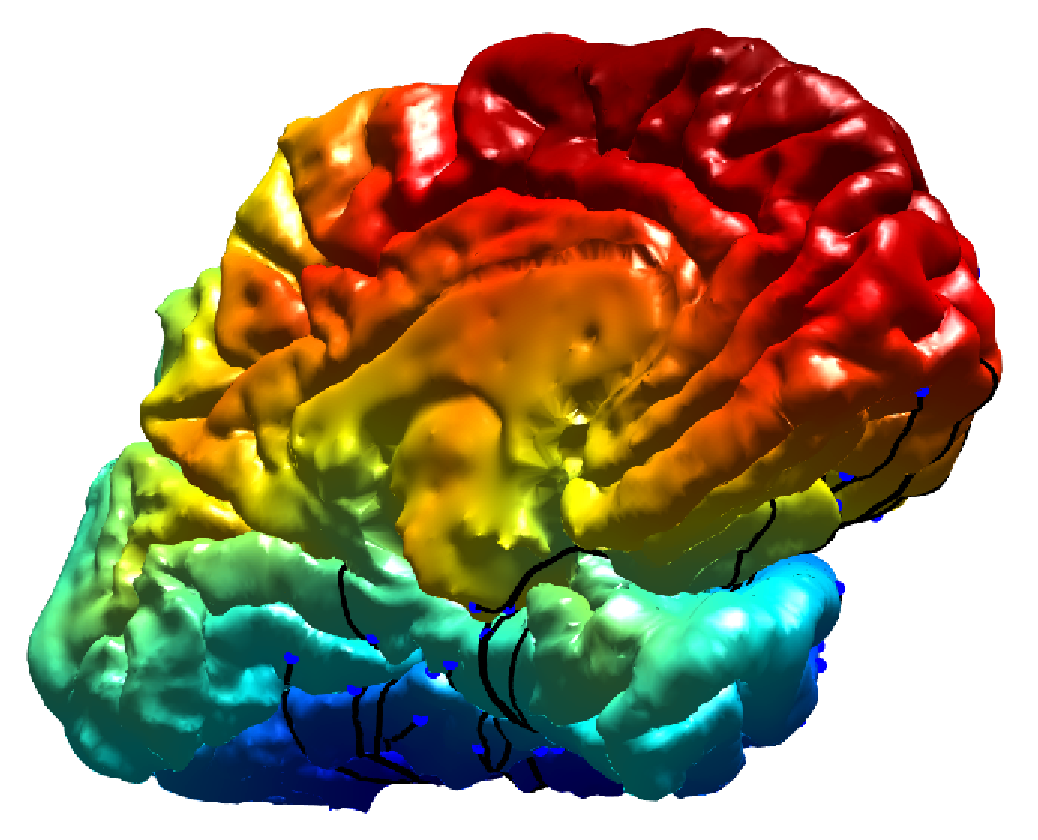
\includegraphics[width=.85\linewidth]{Figures/IR38_54toall_antmed.eps}
        \caption{Medial}
        \label{fig:sfig1}
    \end{subfigure}
    \begin{subfigure}{.45\textwidth}
    \centering
    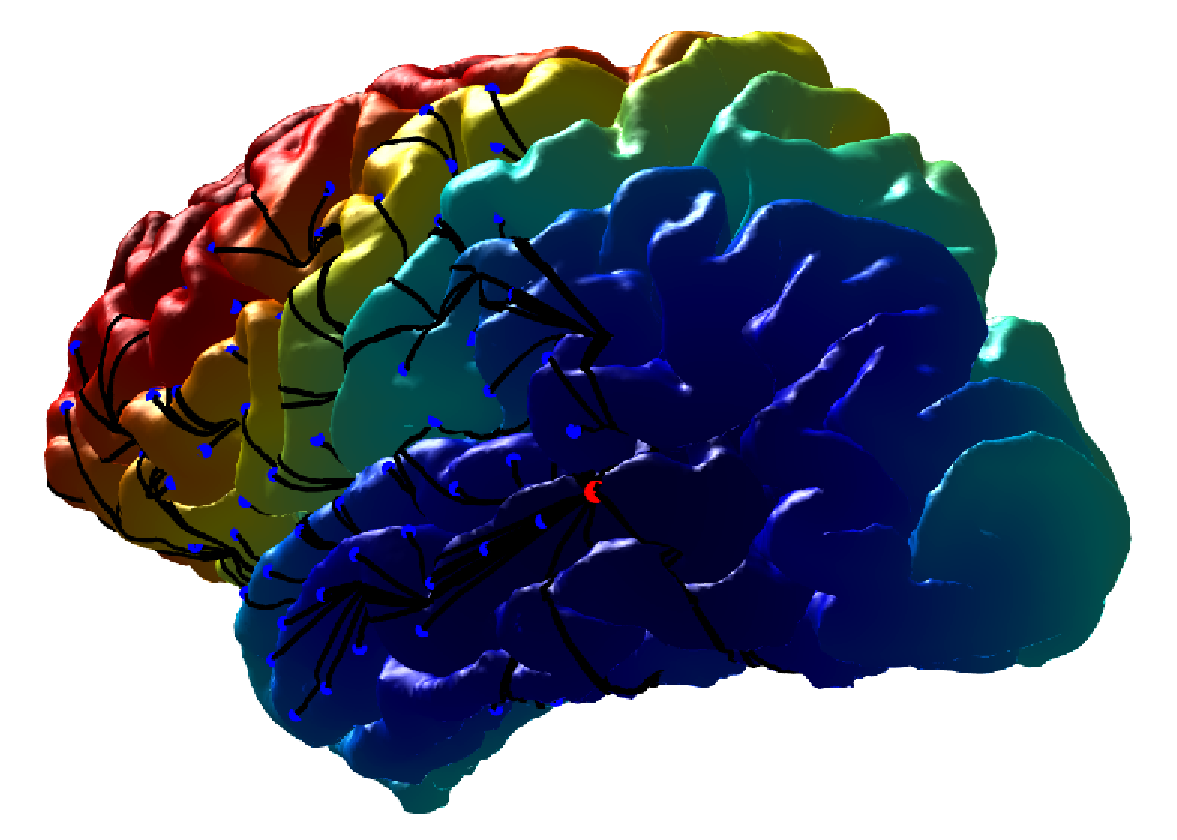
\includegraphics[width=.9\linewidth]{Figures/IR38_54toall_latpost.eps}
        \caption{Lateral}
        \label{fig:sfig2}
    \end{subfigure}
    \caption{Geodesic distances from electrode in red to each vertex of surface mesh. Near to far color scale goes from blue to red}
    \label{fig:GeoDist}
\end{figure}

\begin{figure}
    \begin{subfigure}{.45\textwidth}
    \centering
    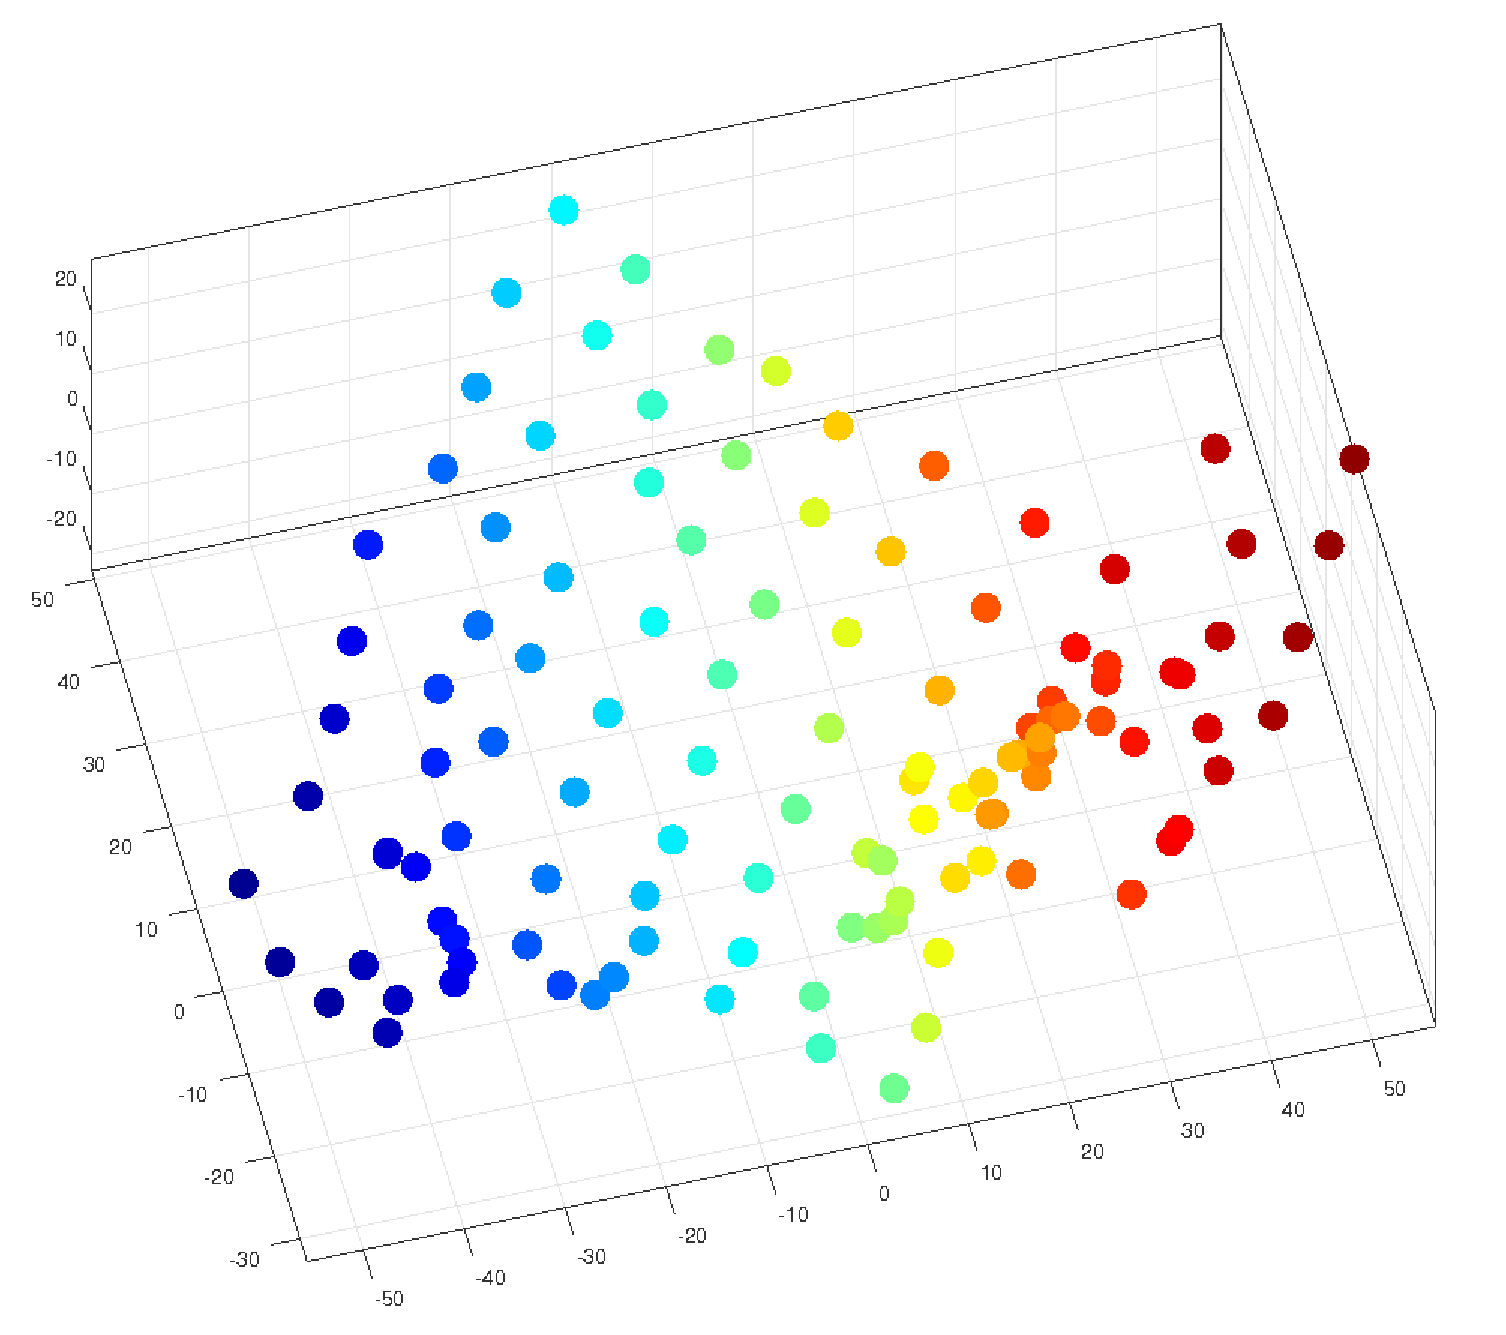
\includegraphics[width=.9\linewidth]{Figures/IR38_MDS_e.eps}
        \caption{Euclidean}
        \label{fig:sfig1}
    \end{subfigure}
    \begin{subfigure}{.45\textwidth}
    \centering
    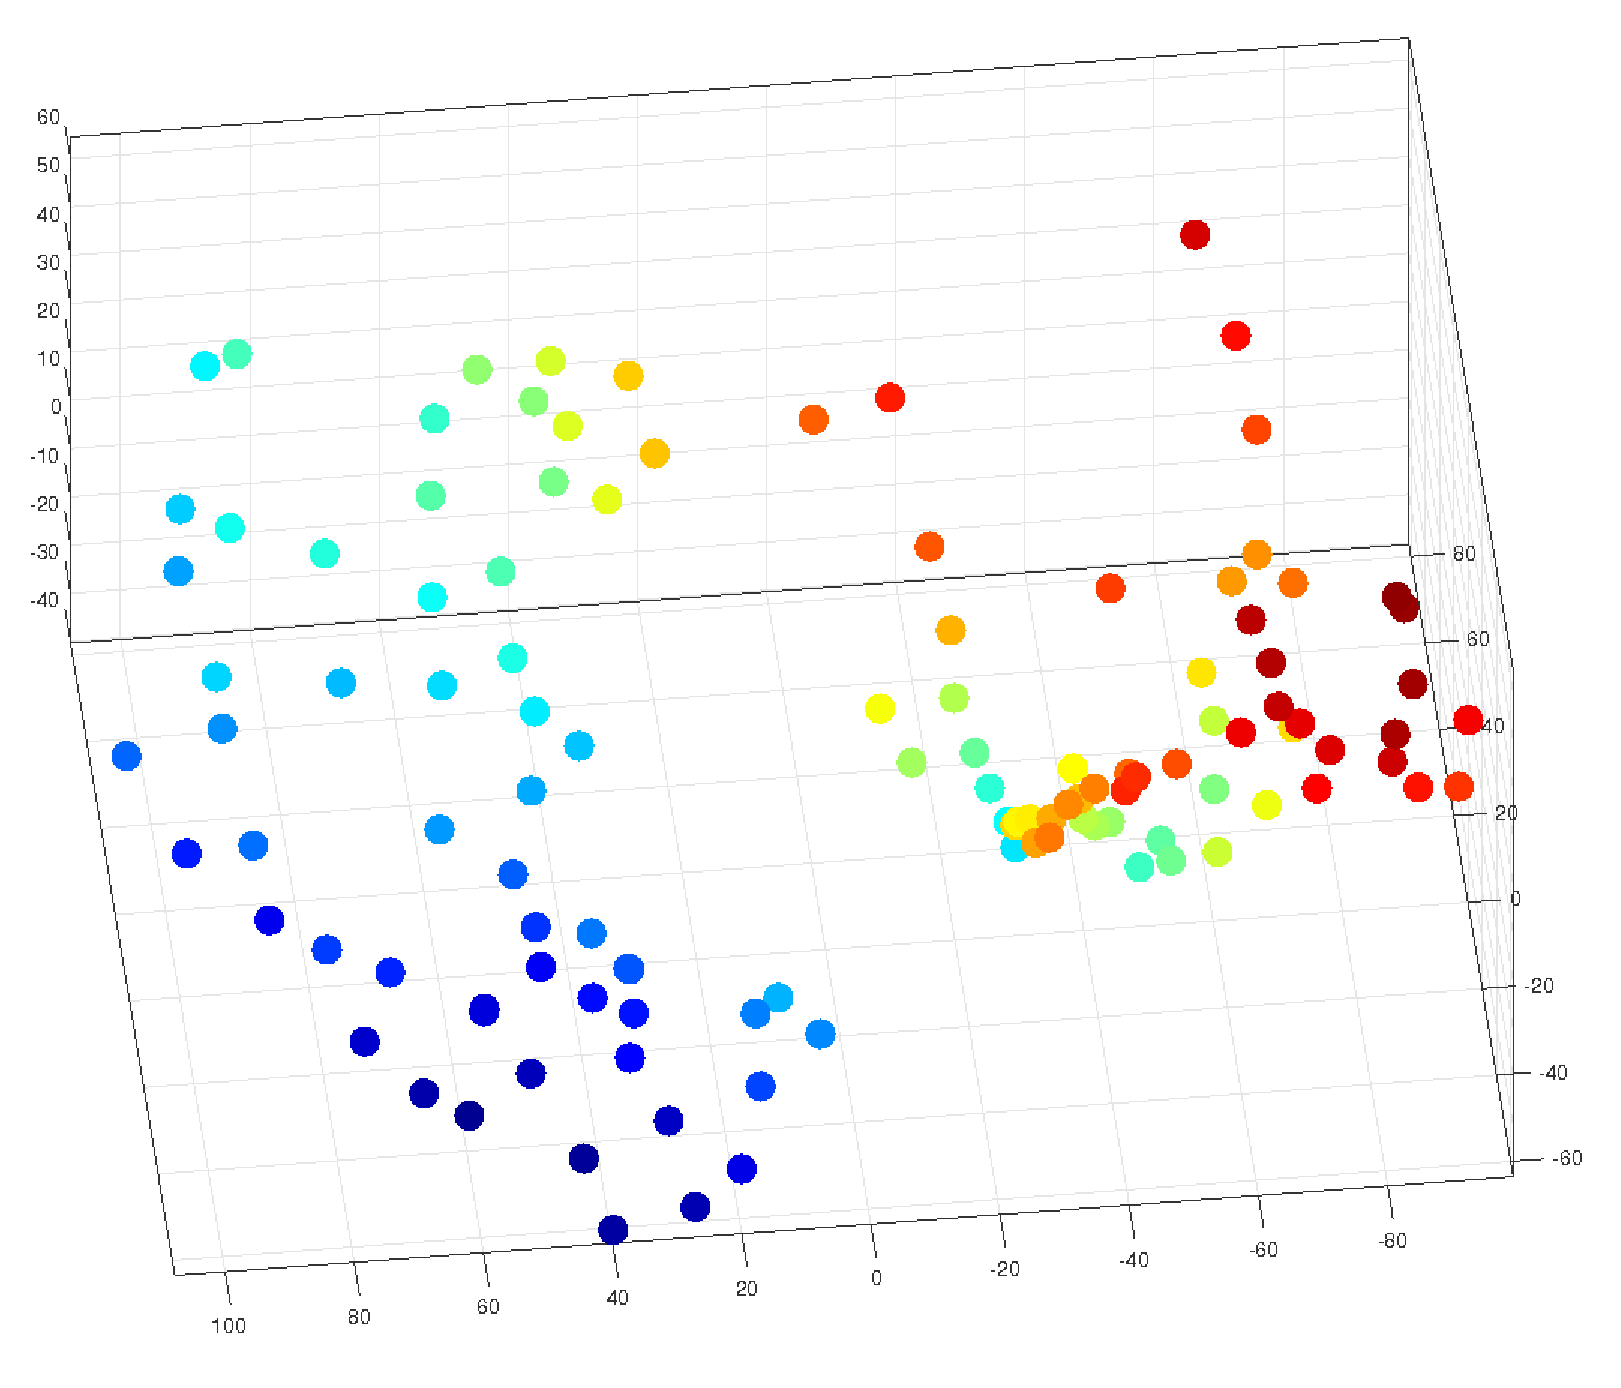
\includegraphics[width=.9\linewidth]{Figures/IR38_MDS_g.eps}
        \caption{Geodesic}
        \label{fig:sfig2}
    \end{subfigure}
    \caption{Multidimensional scaling }
    \label{fig:GeoDist}
\end{figure}


% \subsubsection*{Lag time network}
% Peak lag. Lag of maximum correlation. 

%\section*{Dynamic mode decomposition}
%Another method to reveal structure in multivariate data and reduce dimensionality is dynamic mode decomposition (DMD) \citep{Brunton2016}. 
%[Equations]
%Essentially DMD finds approximate solutions for a first order linear ODE representing each electrode, or the naïve autoregressive model. Each dynamic mode consists of a complex eigenvalue and eigenvector which specifies a complex exponential function over the electrodes. The real part of the eigenvalue determines the exponential growth/decay, and the imaginary part determines its frequency of oscillation, and each complex element of the eigenvector determines the power and phase shift for each electrode. The brain is often described as operating at a critical stability regime, evolving through a sequence of pseudo-steady states. On short timescales, the brain exhibits oscillatory activity, and likewise, DMD on these short windows will reveal oscillatory activity, while on long timescales, the modes will only be trivially stable.
%This short-coming led to a variant called multi-resolution DMD, which can resolve transient modes of activity. This method can be applied to find how the electrodes couple over time in a variety of ways. It can be performed on the entire dataset or intervals defined by various criteria like amplitude, waveform detections, the data can also be spatially filtered for example intervals when hippocampal electrodes are active. For stereotypical activity, it can be applied over all such intervals, or for temporal specificity I could be done on individual intervals, and for even more temporal resolution it can be applied on sub-intervals.

\subsection*{Quantifying spatial dependence of signals}
To determine the spatial dependence of neural signals, we used multiple linear regression generalized for complex arguments to regress a signal into space. Mathematically for a vector of N signals, $s$, at time t, in which each $s_i$, $i \in N$, is located at coordinates $(x_i,y_i,z_i)$,

$$s_i(t) = \beta_0 + \beta_x x_i + \beta_y y_i + \beta_z z_i + \varepsilon_i,$$ 
or
$$s(t) = \hat{\beta}X + \varepsilon,$$

where $\hat{\beta} = [\beta_0, \beta_x, \beta_y, \beta_z]$ and $X_i = [1,x_i,y_i,z_i].$

The beta values for this linear system can be solved for complex components with,

$$\hat\beta = \left(X^*X\right)^{-1}X^* z,$$

where $X^* = \bar{X}^T$, i.e., the complex conjugate transpose.

This enabled us to regress various components of a signals; in particular, (1) real amplitude, (2) complex amplitude, (3) power, and (4) phase. The result of this regression on a set of spatially embedded signal values at given point in time, are three beta values determining a slope in each cardinal direction, and a bias, or intercept, term. Therefore, this method reduces a potentially large set of data to four parameters indicating the direction and average value, i.e. a 4D hyperplane.

To quantify the goodness of fit, the standard $R^2$, explained variance was used. However, to determine if this fit implied that the signals exhibited significant spatial dependence, we employed a bootstrap procedure: identical signal values were regressed after shuffling electrode coordinates and computing $R_{surr}^2$ and this was repeated 100 times to form a surrogate distribution of $R_{surr}^2$ values which were used as a confidence interval for the original $R^2$. Thus, if $R^2$ was greater than all of the $R_{surr}^2$ values, it indicated that the signals had a significant dependence on the original spatial embedding.   

\subsection*{Spatial windowing}
The approach discussed above is limited by fitting only a single model to all channels, which can not capture signal propagation in more than one direction. However, it can be extended using a windowing approach. I implemented such an approach by first grouping electrodes into clusters using the K-nearest neighbors algorithm and subsequently using the regression described above separately on each cluster. However, the benefits of this windowing come at the expense of introducing four more parameters for each additional window.


%\subsection*{Wave propagation}
%These methods effectively approximate the spatial gradient for local to global continuum. Since, wave propagation involves changes in spatial gradient over time, so to infer propagation this    

%\subsection*{Similarity of propagations}
%While propagation. Determining the similarity of propagation events can be reduced to quantifying the similarity of model coefficients. 

\section*{Results}
%The dynamic modes meaningfully reduce the dimensionality of the data into modes of activity across the electrodes, and even more interestingly, these modes tend to be spatially correlated. To ensure this correlation exists, I also compute the spatial correlation on the data filtered for the specific activity.
\subsection*{Brain activity is significantly correlated over space}
In human intracranial recordings during spontaneous sleep, we asked if there was a spatial dependence of these signals.

\section*{Discussion}
Local vs global activity.

Conduction of an electrical wave through a dielectric is a linear process so linear regression is an appropriate method.

One development offered by the current technique is the ability to detect traveling waves in spaces more relevant to brain anatomy as opposed to a Euclidean space defined by the recording array. Geodesic distance is more relevant to brain communication. However, any distance metric could be substituted.
Previous methods used circular statistics and regression techniques, and notably, circular regression does not have a closed-form solution, thus requiring optimization techniques to solve. By using regression generalized for complex arguments, we avoid the need for optimization algorithms, and greatly reduce computation. This enabled us to regress various signals on space using the same method including the (1) real amplitude, (2) complex, (3) power, and (4) phase signals for each band. The present method can be applied to any number of recording locations in time. However, it is possible that multiple waves are present in the data. 


%% Trash

    % \begin{subfloat}{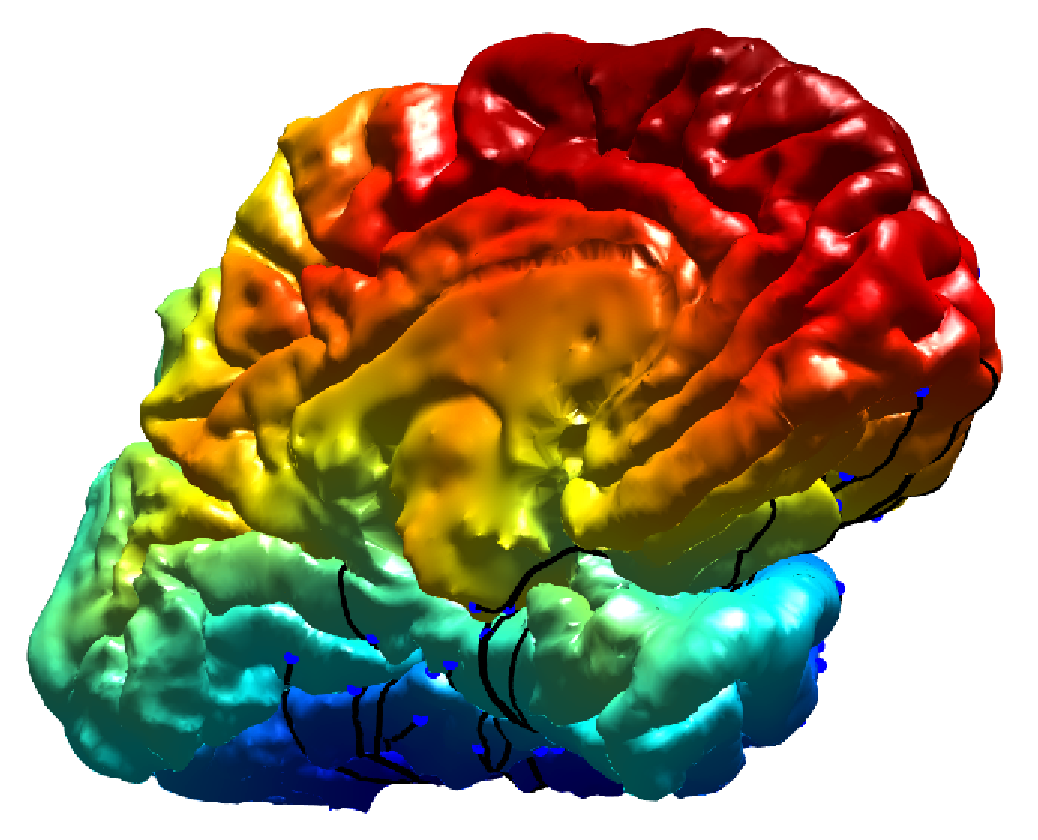
\includegraphics[scale=.2]{Figures/IR38_54toall_antmed.eps}}
    %     \caption{Anterior-medial}
    %     \label{fig:sfig1}
    % \end{subfloat}
    % \begin{subfloat}{
\includegraphics[scale=.2]{Figures/IR38_54toall_inf.eps}}
    %     \caption{Inferior}
    %     \label{fig:sfig2}
    % \end{subfloat}
    % \begin{subfloat}{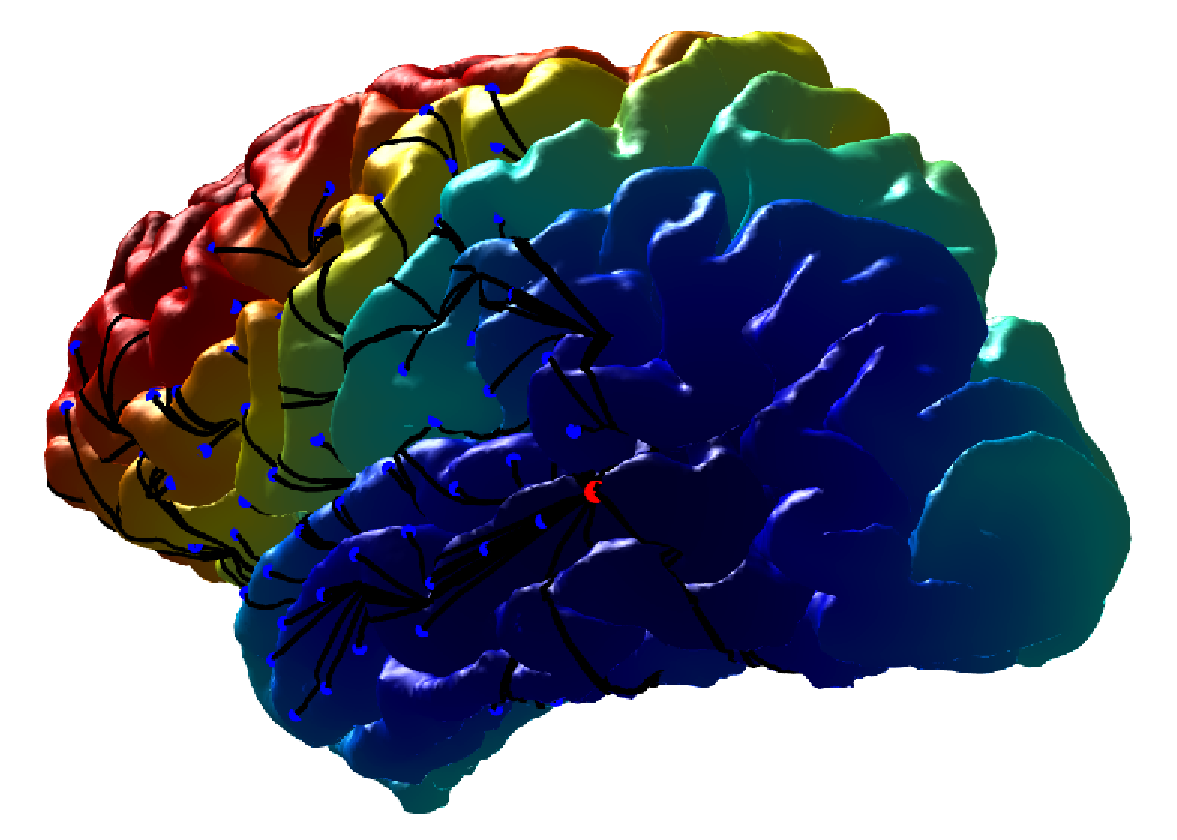
\includegraphics[scale=.2]{Figures/IR38_54toall_latpost.eps}}
    %     \caption{Posterior-lateral}
    %     \label{fig:sfig3}
    % \end{subfloat}
    
   %Importantly, while the previous method produces a single linear model, i.e. a hyperplane through the origin, this extension produces a composite mode consisting of many affine models, i.e. hyper planes at a distance from the origin, allowing for much more accurate fits. 
   
%%% Local Variables: ***
%%% mode: latex ***
%%% TeX-master: "thesis.tex" ***
%%% End: ***
